\documentclass[journal,onecolumn,11pt]{IEEEtran} 
\ifCLASSINFOpdf
  % \usepackage[pdftex]{graphicx}
  % declare the path(s) where your graphic files are
  % \graphicspath{{../pdf/}{../jpeg/}}
  % and their extensions so you won't have to specify these with
  % every instance of \includegraphics
  % \DeclareGraphicsExtensions{.pdf,.jpeg,.png}
\else
  % or other class option (dvipsone, dvipdf, if not using dvips). graphicx
  % will default to the driver specified in the system graphics.cfg if no
  % driver is specified.
  % \usepackage[dvips]{graphicx}
  % declare the path(s) where your graphic files are
  % \graphicspath{{../eps/}}
  % and their extensions so you won't have to specify these with
  % every instance of \includegraphics
  % \DeclareGraphicsExtensions{.eps}
\fi

% packages added by fzen
\usepackage{graphicx}
\usepackage{sidecap}
\usepackage{color}
\usepackage{glossaries}
\usepackage{comment}
\usepackage[margin=1.25in]{geometry}
\geometry{top=1in, left=1.25in, right=1.25in, bottom=1in}
\usepackage{setspace}
\doublespacing
% \usepackage[square, comma, sort&compress]{natbib}

% Define acronymns
% \makeglossary
\newacronym{sg}{SG}{surrogate gradient}
\newacronym{ann}{ANN}{artificial neural network}
\newacronym{rnn}{RNN}{recurrent neural network}
\newacronym{snn}{SNN}{spiking neural network}
\newacronym{stdp}{STDP}{spike timing-dependent plasticity}
\newacronym{bptt}{BPTT}{back-propagation through time}
\newacronym{rtrl}{RTRL}{real-time recurrent learning}
\newacronym{lel}{LEL}{local error learning}
\newacronym{lif}{LIF}{learky integrate-and-fire}
\newcommand{\HM}[1]{\textcolor{red}{{\bf HM:}~#1}}

\begin{document}

\title{Learning to Solve Real-World Problems with Spiking Neural Networks}
% Other possible titles
% \title{Surrogate-gradient-descent learning in spiking neural networks}

\author{Emre O. Neftci$^\dagger$,~\IEEEmembership{Member,~IEEE,}
        Hesham Mostafa$^\dagger$,~\IEEEmembership{Member,~IEEE,}
        Friedemann Zenke$^\dagger$\\
        {\small $^\dagger$ All authors contributed equally. The order of authors is random.}}% <-this % stops a space
\markboth{IEEE SPM White Paper for the special issue on neuromorphic computing}%
{}
%
\maketitle
\IEEEpeerreviewmaketitle
%
\begin{abstract}
A growing number of neuromorphic \gls{snn} processors that emulate biological neural networks are creating an imminent need for methods and tools enabling them to solve real-world problems involving real-time signal processing.
Like conventional neural networks, \glspl{snn} are particularly efficient when trained on real, domain specific data. 
However, their training requires overcoming a number of challenges linked to their binary and dynamical nature.
This tutorial elucidates step-by-step the challenges typically encountered when training \glspl{snn}, and guides the reader through the key concepts of synaptic plasticity and data-driven learning in the spiking setting.
In so doing, it introduces surrogate gradient methods as a particularly flexible and efficient method to overcome the aforementioned challenges and discusses the ``tricks of the trade''. 
\end{abstract}

\section{Introduction}
%%I think we should start with brain inspiration. The special issue is about brain-inspires computing. 
\textbf{Add "brain inspiration here"}
% Signal processing introducing
A plethora of signal processing problems are concerned with real-time pattern recognition or noisy time series prediction.
To solve real-world problems with intrinsically nonlinear dynamics and an inherent history dependence, \glspl{rnn} often constitute a viable solution CITE.
However, to deploy \glspl{rnn} two key challenges need to be addressed.
First, before an \gls{rnn} can be used to predict outcomes on new data, it needs to be trained. 
Training is the optimization procedure in which the the parameters or weights of the \gls{rnn} are adjusted to approximate a specific function that the \gls{rnn} is to perform.
Training \glspl{rnn} can be impeded by a variety of factors common for real world applications, e.g.\ noise and non-stationary of the data. 
Overcoming these limitations is an active field of research, many of which have been reviewed in detail elsewhere CITE. % TODO cite a review
Second, power efficiency is an increasingly important issue, especially in embedded and automotive applications, and is becoming an increasing issue as models scale up. % CITE maybe Kwabena's review?
To tackle the latter problem, simplified neural network applications have been devised which are amenable to be run natively on dedicated hardware, such as neuromorphic hardware and neural network accelerators. 
For instance, one common approach are binary activation neural network implementations which can dispense with energetically costly floating-point multiplications. % CITE
\Glspl{rnn} with a binary activation are called \glspl{snn}.
Thus \glspl{snn} constitute as a subset of conventional neural networks. 
\Glspl{snn} are an area of active study both due to their potential for power efficient computation and more fundamentally because \glspl{snn} are the dominant network model employed by the brain.
% Even in the absence of recurrent connections, recurrence appears due to the dynamical nature of the spiking neuron. 
This tutorial focuses on the key challenges which occur when \glspl{snn} are to solve real-world signal processing problems. 


Two key challenges are the spatial and the temporal credit assignment, i.e.\ how weights and parameters of hidden units need to be modified to improve the objective during training.
Conventional \glspl{rnn} are trained by gradient descent on a scalar objective of loss function. For gradient descent to be a well defined training procedure, \glspl{rnn} are typically designed to be continuously.
This is the main differences to binary and spiking neural networks which whose nonlinearities do not have a smooth continuous derivative. 
% TODO maybe we should have a nice figure for this?

The three most common approaches can be coarsely classified into the following three main categories:
i) resorting to entirely unsupervised learning for the hidden units,
ii) smoothing the network model to be continuously differentiable,
or iii) defining a surrogate gradient as a continuous relaxation of the real gradients.
Approaches pertaining to unsupervised learning has been reviewed extensively in CITE. % TODO insert maida and masquellier arxiv review.
In this tutorial we thus focus on the latter two supervised learning approaches which we will refer to in the following as the ``smoothed'' and \gls{sg} approach for brevity. The main difference between the two is that smoothed approaches entail modifications to the forward pass of the network dynamics by either dispensing with binary nonlinearities or by introducing stochasticity, whereas \gls{sg} leave the forward pass untouched and act solely on the learning dynamics directly. In the following, we briefly discuss common ``smoothing'' approaches before turning to \glspl{sg}.


\section{Smoothed \glspl{snn} (Friedemann)}

The defining characteristic of smoothed \glspl{snn} is that their formulation ensures well-behaved gradients which are directly suitable for optimization. 
Smooth models can be further categorized into soft nonlinearity models and 
probabilistic models. For the latter smooth gradients technically are only defined on expectation values. 
The former approach can in principle be applied directly to all spiking neuron models which explicitly include a smooth spike generating process. This includes, for instance,  the Hodgkin-Huxley, Morris-Lecar, and FitzHugh-Nagumo models. 
However, in practice this approach has only been applied successfully by \cite{Huh_Sejnowski17_graddesc} who used an augmented integrate-and-fire model in which the binary spiking nonlinearity was replaced by an continuous-valued gating function. 
The resulting network thus constitutes a \gls{rnn} which can be optimized using standard methods of backpropagation through time or real-time recurrent learning.
It remains unclear, however, how spike reset dynamics can be coupled into such model.

Probablistic models, on the other hand, have been used more widely in the past ...

% TODO insert long laundry list of models
% 






\section{Surrogate gradient approaches (Friedemann)}

% TODO write section

Most \gls{sg} approaches can be further categorized into models relying on a rate-based and spike-based coding schemes

\begin{comment}
Ideas for credit assignment classification:

* spatial credit assignment
    * back-prop-like
    * random feedback (direct feedback, feedback alignment, etc)
    * local error learning
* temporal credit assignment
    *    back-prop-like, e.g. Bellec et al., SLAYER
    *    forward in time (single hop), e.g. SuperSpike
    *    ignored (I think most rate-based approaches, because essentially assume a temporal steady state)

\end{comment}


%%%%%%%%%%%%% what we had before is below

One popular approach to overcome this problem is to treat spike rate as the information-carrying quantity.
In many practical scenarios, spike rate can depend smoothly on the network parameters, such as synaptic weights, which makes it suitable for efficient gradient-based optimization.
Rate-based approaches can offer good performance, but they are often inefficient. On the one hand, precise estimation of firing rates requires averaging over several spikes. 
Such averaging requires time which can slow down the computation. To some degree this problem can be overcome by spatial averaging over large populations of spiking neurons. However, this comes at the expense of more neurons. 

These temporal and resource limitations can be overcome by instead relying on spike timing as the information-carrying quantity.
In this temporal coding scheme, every spike can carry significantly more information compared to rate-based schemes.
However, the increase in efficiency of the neural code comes with a price. \glspl{snn} relying on individual spikes and their timing are intrinsically hard to optimize.
While a neuron's spike time is a continuous quantity which depends smoothly on the parameters, a discontinuity appears where spikes are either generated or annihilated. This poses a major obstacle for gradient-based techniques because gradients become infinite where the discontinuity appears and vanish otherwise.
One approach to learning in the temporal scheme is a bottom-up one, driven by biologically observations of synaptic plasticity, such as \gls{stdp}.
Their intrinsic timing-dependence does in principle allow them to exploit sub-millisecond temporal features in the spike trains. 
However, these bottom-up methods are ad-hoc, yielding in practice lower performance compared to learning rules derived from first principles in a top-down manner, such as gradient descent.

Continuous relaxations of the spiking neuron dynamics in gradient descent have proven surprisingly effective in improving learning in the temporal coding scheme. There, instead of working with the exact gradient of a non-differentiable spiking threshold, a \emph{Surrogate} Gradient (SG)  is computed from a continuous relaxation of the threshold. 
%%Emre: Let's keep the details out 
%A common choice is, for instance, a sigmoidal nonlinearity. 
%For example, in the limit of infinitely steep slope of the sigmoidal non-linearity, the original hard-threshold behavior of a spiking neuron is recovered.
The use of \glspl{sg} allows to efficiently train \glspl{snn} without specifying whether a temporal or spike-timing based coding scheme is to be used. 
Like vanilla gradient-descent, \gls{sg} learning can deal with the spatial and temporal credit assignment problem by either back-propagation through time or, alternatively, by forward-propagation of all relevant information through eligibility traces. In doing so, \gls{sg} learning can be reduced to local three factor rules which may be more amenable for hardware implementations. 

Based on our recent work, this tutorial details the formulation of \gls{sg} descent algorithms for training multilayer \glspl{snn}, and their application to feature learning in the spiking domain.
We show how such learning algorithms provide learning dynamics that are tailored to the neuron's dynamics, and demonstrate a practical use case in adaptive event-driven sensor data processing. 
We discuss the main advantages of \gls{sg} learning compared to other learning methods, namely that 1) they prescribe synaptic plasticity dynamics that are directly anchored in first principles, enabling \glspl{snn} to efficiently optimize formal objective functions, 2) they bridge recent advances in deep learning and \glspl{snn}, and 3) they outperform traditional \gls{snn} training approaches in multilayer or recurrent architectures.  
Finally, this tutorial lays out approaches to prototype efficient learning and inference algorithms in \glspl{snn} with the hardware available to the user, including mixed signal and digital neuromorphic hardware, and existing machine learning software. 

\section{A walk-through example of surrogate gradient descent}

In the following section we will provide a brief walk-through to training a spiking neural network with \gls{sg}.
To that end we will first introduce the \gls{lif} neuron model
with current-based synapses as 
a standard neuron model which finds wide use in computational neuroscience.

Next, we will reformulate this model in discrete time and show its formal equivalence to a discrete time \glspl{rnn} with binary activation function. 
Formulating \glspl{snn} as \glspl{rnn} is a worthwhile conceptional exercise. 
Decades of research in machine learning has endowed us with a rich repertoire of methods and tools to efficiently train \gls{rnn}.
% TODO write here 


it allows us to directly transfer a body of knowledge on how to obtain gradients for \glspl{rnn} can readily be obtained by dint of \gls{bptt} or \gls{rtrl}. % TODO REFS


% Introduce LIF in differential form
We begin by noting that a single \gls{lif} neuron, a standard neuron model which is widely used in computational neuroscience, can be interpreted as a simple \gls{rnn}. 
A \gls{lif} neuron can be formally be described in differential form as
\begin{equation}
    \tau_\mathrm{mem} \frac{dU}{dt} = -U + RI
\end{equation}
where $U(t)$ is the membrane voltage, which describes the state of the neuron, $\tau_\mathrm{mem}$ is the membrane time constant, $R$ is the input resistance, and $I(t)$ is the input current.
It is easy to see that $U$ acts as a leaky integrator of the input current $I$.

In spiking neural networks the input current is typically generated by synaptic currents that are triggered by the arrival of presynaptic spikes $S_j(t)$.
When working with differential equations, it is convenient to denote a spike train $S_j$ as a sum of Dirac delta functions
$$S_j(t)=\sum_k \delta(t-t_j^k) \quad .$$
This will become important later.

Synaptic currents have temporal dynamics themselves. A reasonable first approximation is to model their time course as an exponential current following each presynaptic spike. Moreover, synaptic currents sum linearly, thus we can write:
\begin{equation}
    \frac{dI}{dt}= -\frac{I(t)}{\tau_\mathrm{syn}} + \sum_j W_j S_j(t)
\end{equation}
where the sum runs over all presynaptic neurons $j$.
Taken together 

% Formulate model in discrete time



% Formulate as network -- trivial
\begin{figure}
    \centering
    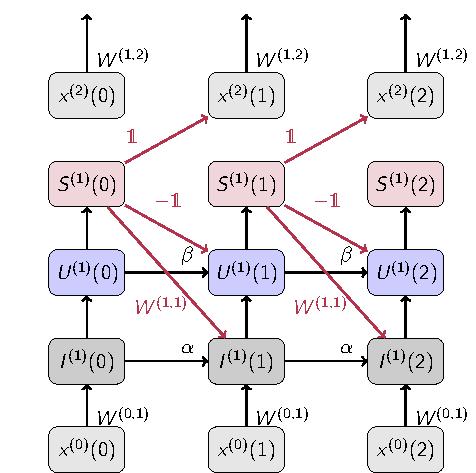
\includegraphics{figures/snn_graph.pdf}
    \caption{Caption}
    \label{fig:snn_compgraph}
\end{figure}



\section{Credit Assignment}
In gradient-based learning, the parameter updates contain a term that relates to the local error or, more generally, the derivative of the loss. In a neural network, this term is affected by the computations downstream from the updated node. This is the credit assignment problem. In conventional neural networks, the credit assignment problem is solved by backpropagating the errors from the output layer using the chain rule (\emph{i.e.} the gradient BP rule).
The gradient BP rule relies on the immediate availability of backpropagated errors represented with high-precision memory. In conventional computers, the access to this information depends on a memory of that is shared by nodes that are contiguous in the graph.
This type of shared memory does not exist in the brain, as states and parameters are local to the neurons and synapses.
Errors needs to be at the right place at the right time, and do non-locality can be spatial or temporal, or both.
In spatial non-locality, a special communication channel that transmits the errors to the relevant nodes must be provisioned to solve the credit assignment problem \cite{Baldi_Sadowski16_theoloca}. 
In temporal non-locality, some form of (working) memory is required to maintain the history of the relevant states. 
Non-localities, both temporal and spatial, are arguably the most challenging and constraining aspect of spiking neural networks and synaptic plasticity \cite{Neftci18_datapowe}. 
However, non-locality enables a tremendous advantage: massively parallel computing with carefully controlled (and potentially dynamic) interprocess communication. 
Thus, solving the ability to learn and process using local information is not only interesting to neuroscientists: it can enable machine learning accelerators that approach the reliability and energy-efficiency of the brain.
In the following two sections, we describe solutions to the spatial and temporal credit assignment problems in spiking neural networks.

\subsection{Spatial Credit Assignment (Hesham)}

\subsection{Temporal Credit Assignment (Emre)}
Some form of memory is required to solve the credit assignment problem, generally present in recurrent neural networks. 
Generally speaking, this can be achieved in two different ways \cite{Williams_Zipser89_learalgo}:
1) The recurrent neural network is ``unrolled'' meaning that a graph is created by cloning the network for each time step of the system (see figure \ref{fig:snn_compgraph}). This way, the temporal credit assignment problem can be solved by back propagating through the unrolled network. Computationally, this requires maintaining all the inputs and activations for each time step. Thus the memory required using this approach scales as $O(N T)$, where $T$ is the duration of the sequence.
2) The information for computing the errors is propagated forward.
\textbf{Use Williams and Zipser equations, and explain special case where the ODE has a solution = superspike}

Unsurprisingly, both solutions consist in transforming the temporal credit assignment problem to a spatial credit assignment problem.

Learning on a non-local substrate means that the weight updates must be performed in a non-local fashion as well. Importantly, if training is performed epochwise (meaning weights are updated at the end of a sequence), a separate memory is required to accumulate the incremental weight updates. In the equation \ref{eq:integral_superspike}, this memory is implicitly assumed by the integral. Alternatively, the weights can be updated incrementally, meaning a weight update is performed at every time step, or when the instantaneous local error exceeds a threshold as in 
\textbf{Error-triggered learning} \cite{Neftci18_datapowe}.
\textbf{Describe the synchronization effect of incremental learning}.

%\section{Outline}
%%%%%%%% 
%\subsection{Introduction}
%This section covers the key characteristics of biological neural networks  \cite{Gerstner_Kistler02_spikneur}, including their dynamics, their potential for robust coding and efficient communication, and the consequences of computing on a physical substrate. 
%Next, it categorizes existing approaches to train \glspl{snn}, contrasting bottom-up and top-down (normative) theories, temporal vs. rate-based ones, and the capabilities of the state-of-the-art in each category. It will discuss the computational features of \glspl{snn} compared to artificial neural networks, their implementation in hardware, and the promises of \glspl{snn} to advance mobile, automotive and medical technologies.
%
%\subsection{Learning in Computational Neuroscience} 
%{\color{red} Merge with intro section.\\ }
%This section describes formally the traditional learning dynamics used in computational neuroscience, such as Hebbian learning in Hopfield networks, \glspl{stdp} \cite{masquelier_unsupervised_2007, tavanaei_deep_2018}, and reservoir models \cite{Buonomano_Maass09_statcomp,Sussillo_Abbott09_genecohe,Huang_etal06_extrlear}. 
%Following from the categorization in the introduction, this section covers classic gradient-based learning without hidden units, such as learning precisely timed output spike trains \cite{memmesheimer_learning_2014}, ReSuMe \cite{ponulak_supervised_2009}, the Tempotron \cite{Gutig_Sompolinsky06_tempneur}, the Chronotron \cite{florian_chronotron:_2012}. 
%The section continues describing prior approaches to learning with hidden units\cite{gardner_learning_2015}, including SpikeProp \cite{bohte_error-backpropagation_2002}, NormAD \cite{Kulkarni_etal17_learreal}, Spiking Expectation Maximization \cite{Nessler_etal13_bayecomp}, temporal codes for deep learning with spikes \cite{OConnor_Welling16_deepspik}, train-and-transfer techniques \cite{Esser_etal16_convnetw}, and predictive coding \cite{Deneve_etal17_braieffi}.
%% A common limitation in these methods is their inability to solve credit assignment in both temporal and spatial domains in deep networks. Consequently, there is space for improvement for efficient and accurate data-driven learning in \glspl{snn}.
%
%\begin{figure*}
%\centering 
%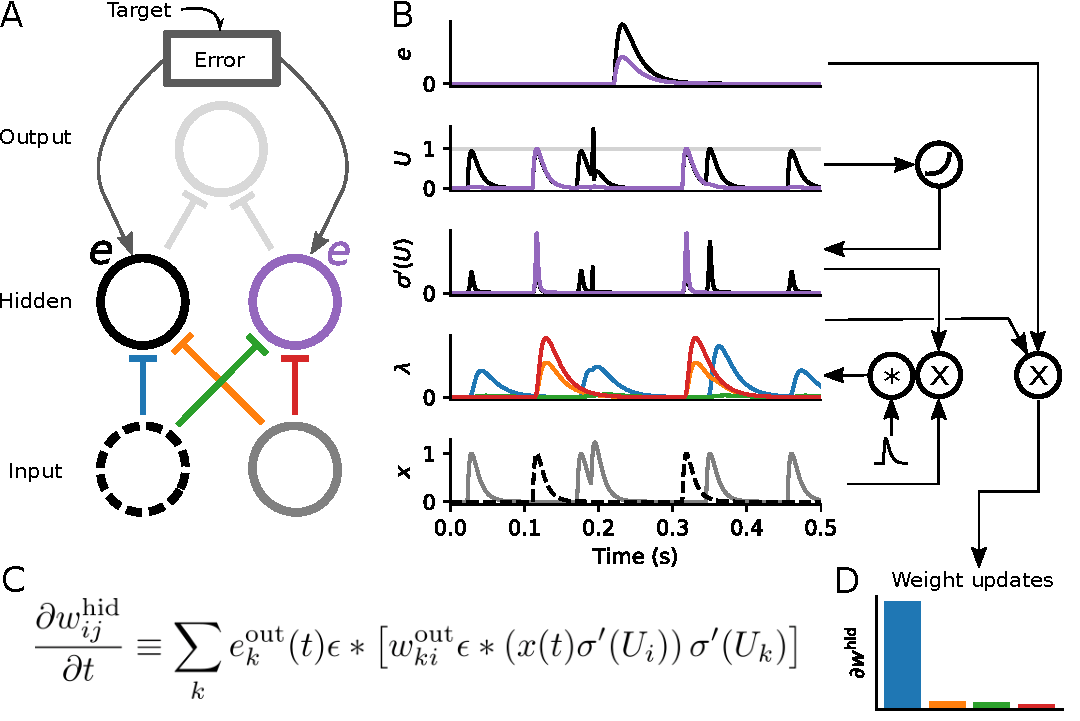
\includegraphics[width=3.0in]{./figures/superspike_concept.pdf}
%\caption{Example of SuperSpike learning of precisely timed target spikes in a three layer network.
%\textbf{A} Illustration of the network layout. Error signals are computed at the top using the van Rossum distance to the target spike train. These error signals are then send to the output unit and the hidden layer units. 
%\textbf{B} Time series of relevant quantities during one learning step. From top to bottom: $e$: The error signals as received by the two hidden units. $U$: The membrane voltage of the hidden units. $\sigma^\prime(U)$: The surrogate gradient for the hidden-layer spike trains ($S(U)$) which is computed from $U$ by applying a suitable monotonic nonlinearity which peaks at the firing threshold. $\lambda$: The four eligibility traces of the four hidden layer synapses. The eligibility traces are obtained by multiplying $x$ and $\sigma^\prime$ and further filtering them with the kernel of the van Rossum distance. $x$: The filtered input spike trains.
%\textbf{C} Weight update rule with symmetric feedback weights and without straight through estimation of downstream activities.
%\textbf{D} Bar chart of the weight updates in this example. The final weight updates are obtained by computing the product of the local error signals $e$ with the corresponding eligibility traces. In this example, increasing the blue synapse would be most beneficial for the network to minimize the output error.
%\label{fig:superspike_concepts}}
%\end{figure*}
%
%\subsection{Gradient-based Learning in \glspl{snn}} 
%This section describes a different type of gradient-based learning that is gaining significant momentum for training deep \glspl{snn} on practical tasks.
%It starts by describing the theory of gradient-based learning in multilayer artificial and biological neural networks \cite{Neftci18_datapowe}, using layman mathematical formulas. It follows with a mathematical description of spike-based computing and its relationship with binary neural networks. In the light of the provided mathematical formulas, the section underlines the physical nature of neural computation, and that, through the concept of the learning channel \cite{Baldi_etal17_learmach},  locality in learning equates with efficiency. Next, the section describes continuous relaxations of \glspl{snn}, namely the \glspl{sg} descent approach (see motivation).
%An overview of important prior work \cite{Esser_etal16_convnetw, courbariaux_binarized_2016, bellec_long_2018} will be following by the authors' related work on this topic, namely Random Backpropagation \cite{Neftci_etal17_evenrand}, Deep local learning \cite{Mostafa_etal17_deepsupe}, their extension to spiking networks using deep continuous local learning (Fig.~\ref{fig:dcll}), and SuperSpike 
%(Fig.~\ref{fig:superspike_concepts}; \cite{zenke_superspike:_2018}).
%Formally, this section concludes by underlining the bridges \glspl{sg} learning offers with the rich literature of machine learning and deep learning, and how this can lead to practical solutions, for example in reinforcement learning.
%
%\subsection{Approaches and tools for simulations and emulations of \glspl{snn}}
%{\color{red} Describe PyTorch and/or Auryn sims here\\ }
%An important obstacle in \glspl{snn} research is the prescription and simulation of large networks capable of solving problems routinely tackled in deep neural networks. This section argues that \gls{sg} learning in SNNs greatly facilitates this endeavor, as it naturally lends itself to the automatic differentiation tools \cite{Neftci18_datapowe} of machine learning frameworks. The section concludes by providing step-by-step instructions for running large-scale (up to 1M neurons) simulations of \glspl{snn} with \gls{sg} learning in pyTorch.
%
%\subsection{Applications and Benchmarks of \glspl{snn}}
%{\color{red} Gear this for signal processing\\ }
%\glspl{snn} can be viewed as a subclass of recurrent artificial neural networks. As such, they are best applied to problems dealing with dynamical environments, and in tasks where privacy and energy are paramount. This section will provide a table of benchmark datasets that are well suited to \glspl{snn}. Furthermore, we will provide a detailed example in DVS sensor data processing (Fig.~{fig:dcll}).
%
%\subsection{Conclusion}
%A brief conclusion summarizing the advantages and disadvantages of \gls{sg} learning compared to other approaches, as well as a vision for learning with \gls{sg}.
%
%\begin{figure*}
%\centering
%% \begin{center}
%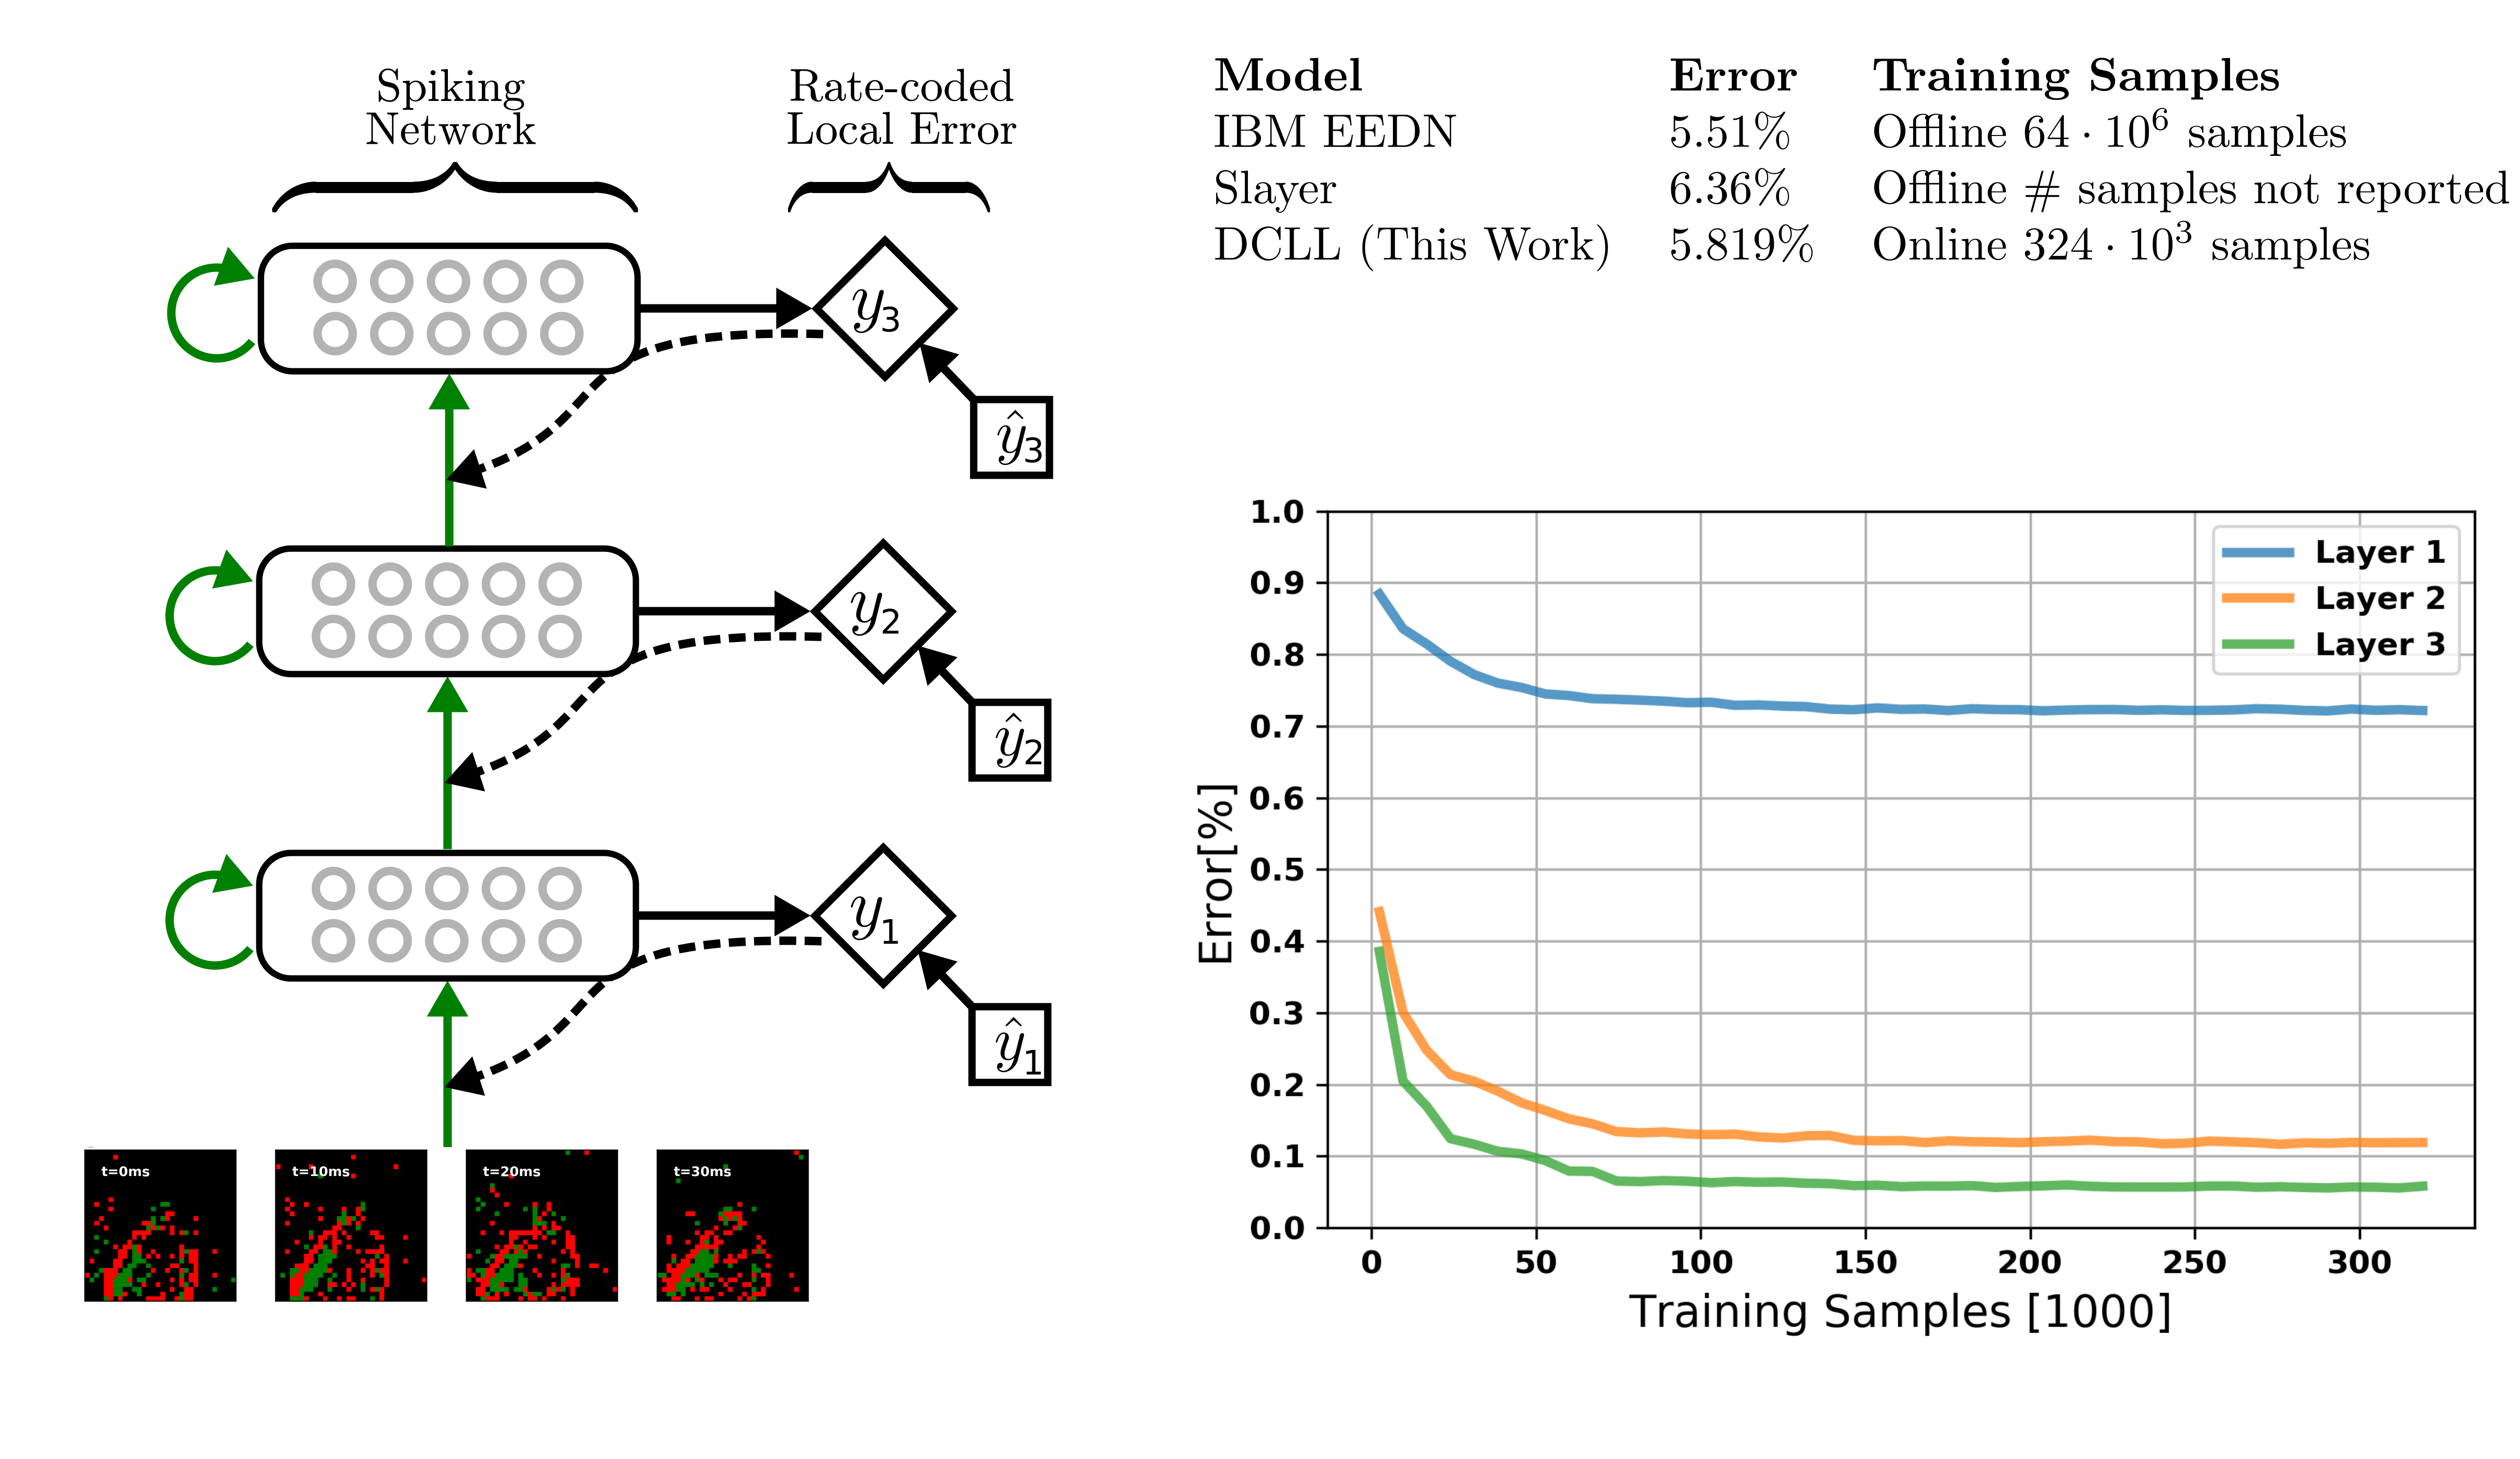
\includegraphics[height=.2\textheight]{./figures/DCLL_illustration.png}
%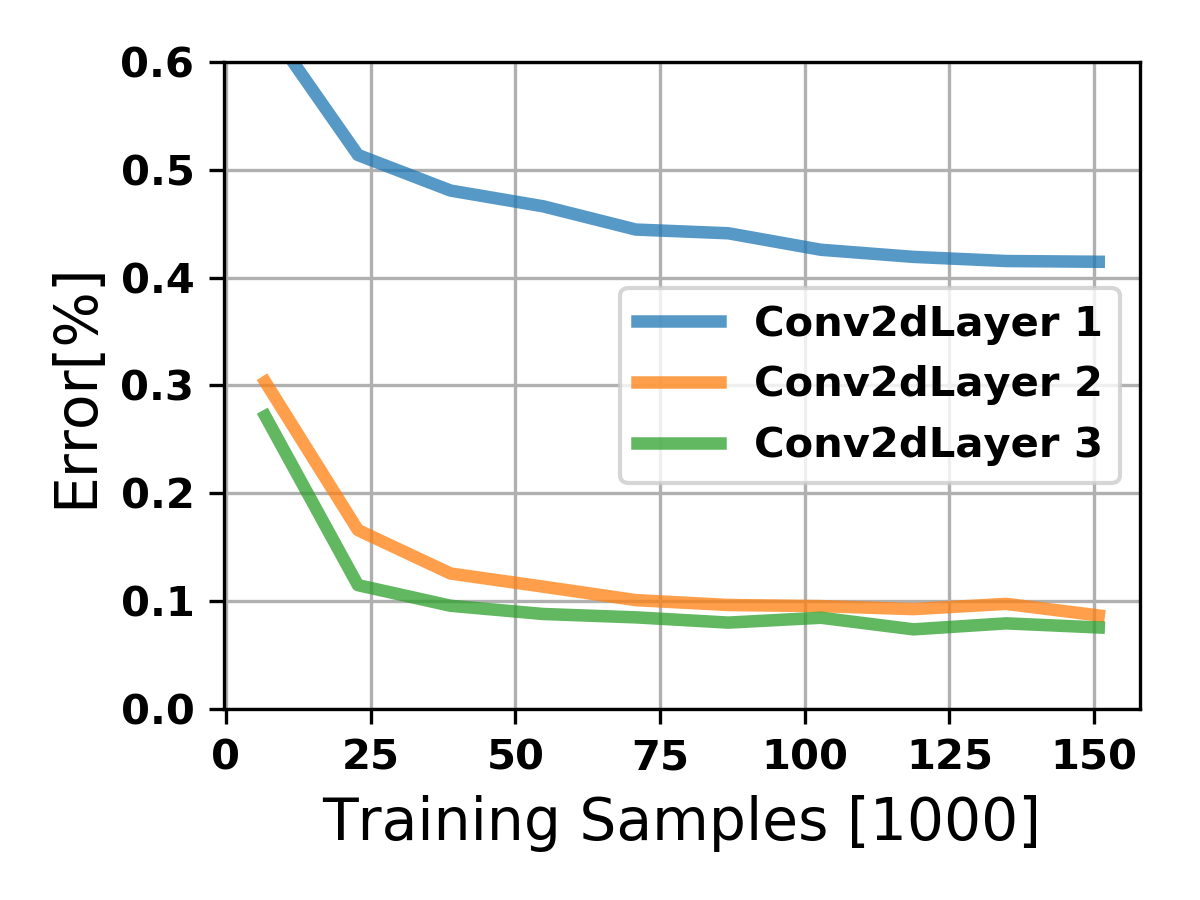
\includegraphics[height=.13\textheight]{./figures/convergence_dvs_gestures_small}
%% \end{center}
%\caption{\label{fig:dcll} Deep Continuous Local Learning (DCLL) with spikes, applied to the DVSGestures dataset. A three layer convolutional spiking neural network is trained with \gls{sg} using local errors generated using fixed random projections to a local classifier. Learning in DCLL scales linearly with the number of neurons thanks to local rate-based cost functions formed by spike-based basis functions. Thanks to the \gls{sg} approach, the plasticity dynamics (dashed line) are synthesized with automatic differentiation under pyTorch. Results here are shown for the DVS Gestures dataset, 11 gestures recorded using a Dynamic Vision Sensor \cite{Amir_etal17_lowpowe}.}
%\end{figure*}




% % Local learning rule Example: SuperSpike
% \paragraph{Stochastic neural networks} \cite{Neftci_etal14_evencont,Neftci17_stocsyna,Neftci_etal17_evenranda}.



% use section* for acknowledgment
% \section*{Acknowledgment}
% This work was partly supported by the Intel Corporation (EN), and the National Science Foundation under grant 1640081 (EN).

% Can use something like this to put references on a page
% by themselves when using endfloat and the captionsoff option.
% \ifCLASSOPTIONcaptionsoff
%   \newpage
% \fi


\bibliographystyle{IEEEtran}
\bibliography{biblio_unique_alt}

\section{Author Information}
\textbf{Emre Neftci, UC Irvine (eneftci@uci.edu)}\\
Dr.~Neftci is an assistant professor in the department of Cognitive Sciences and Computer Science at UC Irvine. He received his masters degree in Physics at Ecole Polytechnique Federal de Lausanne (EPFL) and his PhD in Neuroinformatics from the Institute of Neuroinformatics at the university of Zurich and ETH Zurich in neuromorphic engineering. His current research explores the bridges between neuroscience and machine learning, with the focus of theoretical and computational modeling of learning algorithms that are best suited to neuromorphic hardware and non-von Neumann computing architectures.\\

\textbf{Hesham Mostafa, UCSD (hmmostafa@ucsd.edu)}\\
Dr.~Mostafa obtained a master's degree in electrical engineering from the Technical University of Munich in 2010, and a PhD in Neuroinformatics from the Institute of Neuroinformatics at the university of Zurich and ETH Zurich. He is currently a post-doc at the integrated systems neuro-engineering lab at the Institute of Neural Computation at University of California San Diego. His research interests include combining ideas from machine learning and computational neuroscience for developing biologically-inspired and hardware-efficient learning and optimization algorithms, and physically implementing these algorithms using CMOS and novel device technologies.  \\

\textbf{Friedemann Zenke, University of Oxford (friedemann.zenke@cncb.ox.ac.uk)}\\
Dr.~Zenke is a Sir Henry Wellcome post-doctoral fellow at the University of Oxford.
He studied physics at the University of Bonn, Germany and at the Australian National University in Canberra. He received his PhD in the laboratory of Wulfram Gerstner at the EPFL where he studied the interaction of synaptic and homeostatic plasticity in spiking neural network models. He then joined the laboratory of Surya Ganguli at Stanford University as a post-doctoral fellow where he used machine learning approaches to explore learning and memory formation in biologically inspired neural networks. He currently continues this line of research in Tim Vogels' Lab in Oxford.






% %%%%%%%%%%%%%%%%
% \cleardoublepage


% % SuperSpike blurp
% SuperSpike is a voltage-based three factor learning rule which can be run on-line. Instead of back-propagation through time, SuperSpike uses biologically plausible synaptic eligibility traces to deal with the temporal credit assignment problem. 




% \section{Skype Notes}
% \begin{enumerate}
% \item intro to \glspl{snn}, what they are
% \item \glspl{snn}, why is it hard.
% \item Comparison/bridge between artificial neural networks. (table) comparisons with random recurrent neural network.
% \item Bottom-up versus top-down / normative.
% \item Surrogate gradient
% \item What sets us apart from Clopath: learning with hidden units. Layered structure. (Gutig also works on simple, single layer networks). Gradient-based learning. Networks that learn from data and structure and generalize from it.
% \item Machine learning frameworks are great. 
% \item Solve credit assignment problem in space and time.
% \item Surrogate-gradient-based (coin a word?)
% \item Local classifier (spiking version)
% \item Tricks of the trade. Regularization, initialization.
% \item Different types of cost functions. eg we don't care about precise spike timing for classification. How to benchmark.
% \item tasks that SNN excel at is different.
% \item recurrent neural network (?)
% \item Boltzmann machines (?)
% \item Spiking VAE (?)
% \item Training networks on-line. forward in time.
% \end{enumerate}



\end{document}